\documentclass[10pt]{beamer}\usepackage[]{graphicx}\usepackage[]{color}
%% maxwidth is the original width if it is less than linewidth
%% otherwise use linewidth (to make sure the graphics do not exceed the margin)
\makeatletter
\def\maxwidth{ %
  \ifdim\Gin@nat@width>\linewidth
    \linewidth
  \else
    \Gin@nat@width
  \fi
}
\makeatother

\definecolor{fgcolor}{rgb}{0.345, 0.345, 0.345}
\newcommand{\hlnum}[1]{\textcolor[rgb]{0.686,0.059,0.569}{#1}}%
\newcommand{\hlstr}[1]{\textcolor[rgb]{0.192,0.494,0.8}{#1}}%
\newcommand{\hlcom}[1]{\textcolor[rgb]{0.678,0.584,0.686}{\textit{#1}}}%
\newcommand{\hlopt}[1]{\textcolor[rgb]{0,0,0}{#1}}%
\newcommand{\hlstd}[1]{\textcolor[rgb]{0.345,0.345,0.345}{#1}}%
\newcommand{\hlkwa}[1]{\textcolor[rgb]{0.161,0.373,0.58}{\textbf{#1}}}%
\newcommand{\hlkwb}[1]{\textcolor[rgb]{0.69,0.353,0.396}{#1}}%
\newcommand{\hlkwc}[1]{\textcolor[rgb]{0.333,0.667,0.333}{#1}}%
\newcommand{\hlkwd}[1]{\textcolor[rgb]{0.737,0.353,0.396}{\textbf{#1}}}%

\usepackage{framed}
\makeatletter
\newenvironment{kframe}{%
 \def\at@end@of@kframe{}%
 \ifinner\ifhmode%
  \def\at@end@of@kframe{\end{minipage}}%
  \begin{minipage}{\columnwidth}%
 \fi\fi%
 \def\FrameCommand##1{\hskip\@totalleftmargin \hskip-\fboxsep
 \colorbox{shadecolor}{##1}\hskip-\fboxsep
     % There is no \\@totalrightmargin, so:
     \hskip-\linewidth \hskip-\@totalleftmargin \hskip\columnwidth}%
 \MakeFramed {\advance\hsize-\width
   \@totalleftmargin\z@ \linewidth\hsize
   \@setminipage}}%
 {\par\unskip\endMakeFramed%
 \at@end@of@kframe}
\makeatother

\definecolor{shadecolor}{rgb}{.97, .97, .97}
\definecolor{messagecolor}{rgb}{0, 0, 0}
\definecolor{warningcolor}{rgb}{1, 0, 1}
\definecolor{errorcolor}{rgb}{1, 0, 0}
\newenvironment{knitrout}{}{} % an empty environment to be redefined in TeX

\usepackage{alltt}
%\usepackage[T1]{fontenc}
%\setcounter{secnumdepth}{3}
%\setcounter{tocdepth}{3}
%\usepackage{url}
%\usepackage{graphicx} 
\usepackage{tikz}

\usetheme{Singapore}
\useoutertheme{miniframes,smoothbars}
\IfFileExists{upquote.sty}{\usepackage{upquote}}{}
\begin{document}

\title{Process control in NGS quality control data}  
\subtitle{Master Thesis, Stockholm University}
\author{Erik Thors\'{e}n}
\date{\today} 

\begin{frame}
\titlepage
\end{frame}

\begin{frame}
  \frametitle{Overview}
  \tableofcontents
\end{frame}

\section{Introduction}
%
% What should be in this section?
% A introduction to the problem
% A introduction on how to solve it
% 
\begin{frame}\frametitle{Aim}
\begin{center}
Construct models which can detect (without our supervision) reduced, or perhaps increased, quality in quality control sequencing data!
\end{center} 
\end{frame}
\begin{frame}\frametitle{Problem description}

\begin{center}
To detect changes and trends in NGS quality control data over time. 
\end{center}

\begin{itemize}
\item Can we deduce a bad/good flowcell from quality control data?
\item Can we detect when the machine is in need of maintainance?
\item If a persistent change occured, can we estimate \textit{when}?
\end{itemize}
\end{frame}


\begin{frame}\frametitle{Types of changes and a solution}
We are interested in the following changes:
\begin{itemize}
\item Transient and large (poor/good sample/flowcell)
\item Persistent and small (ex. machine is in need of maintainance)
\end{itemize}
\pause

\textbf{Solution:}
\begin{center}
\textbf{Statistical process control} and a \textbf{Change-point detection model} 
\end{center}
\end{frame}

% A extended EDA, what should be here?
% Everything that is done for the HiSeq 6 and more!

\section[SPC - models]{Statistical process control - Introduction: Terminology and models}

\begin{frame}\frametitle{Distribution assumption, Machine profile}
\textbf{Assumption 1}: Data follows a multivariate normal distribution.
\begin{center}
$\mathbf{X} \sim \mathcal{N}_p(\boldsymbol{\mu}_0, \Sigma_0)$.
\end{center}
In control machine profile: $\boldsymbol{\mu}_0,\; \Sigma_0$. Machine profile based on quality control data.

\textbf{Assumption 2}: Observations are independent!
\end{frame}

\begin{frame}\frametitle{Statistical process control - Hotellings, MCUSUM, CPD}
Monitor profile $\boldsymbol{\mu}_0, \Sigma_0$ with models:
 \begin{itemize}
 \item Hotelling $T^2$ statistic - large and transient changes (due to poor samples)
 \item MCUSUM scheme - small and persistent changes (due to new parts)
 \item Change point detection (CPD) - \textit{when} did the persistent change occur?
 \end{itemize}
All control charts are directionally invariant $\rightarrow$ only matters that a change occur, not how! 
\end{frame}

\begin{frame}\frametitle{Terminology}
Terminology:
 \begin{itemize}
 \item ARL$_0$ - kind of type 1 error. ARL$_0 \; \leftrightarrow \; 1/\alpha$.
 \item Control limit - a quantile, anything above it is ''extreme''
 \item Allowance constant $k$ - how much variation can we allow? $\uparrow\; k\; \rightarrow$ more variation ok.
 \item For simulations/stress testing:
 \begin{itemize}
 \item ARL$_1$ - kind of the power of a test. ARL$_1 \; \leftrightarrow \; 1/\beta$.
 \item ED - expected delay, like ARL$_1$ but change later ''a delay''. Small=good
 \end{itemize}
 \end{itemize}
 \end{frame}

\begin{frame}\frametitle{How to fit the models}
\begin{enumerate}
\item Estimate or specify machine profile, $\boldsymbol{\mu}_0$ and $\Sigma_0$.
\item Choose type 1 error = choose ARL$_0$. ex. ARL$_0 = 100\; \leftrightarrow \; \alpha=0.01$.
\item Choose $k$. ex. k = 0.3, 0.4 or 0.5
\item Do a lot of simulations to find control limit which fulfills ARL$_0$.
\end{enumerate}
Number of simulations should be large, ex $10^6$. 

\end{frame}

\section[ Desc. of data + EDA]{Description of the data and Exploratory data analysis}
\begin{frame}\frametitle{Description of the data}
Data from 2012 until beginning of 2016. 2012 removed, poor/odd quality control data. 11 operational NGS machines with different characteristics under different run settings. 
\begin{itemize}
\item Two datasets - Tag- and Read level measurements. 
\begin{itemize}
\item Tag level - several measurement per read, one measurement for each tag 
\item Read level - one measurement per read: Multivariate distribution.
\end{itemize}
\item $9$ different quality variables (mean q, error rate,\%tag error, completed run cycles etc.)
\item A Hierachical structure of the flowcells and also a hierachical structure of the machines
\end{itemize}
A total of $801$ unique flowcells. Single read/Paired end
\end{frame}

\begin{frame}\frametitle{Hierachical structure of the data}
\begin{center}
\begin{figure}[!ht]
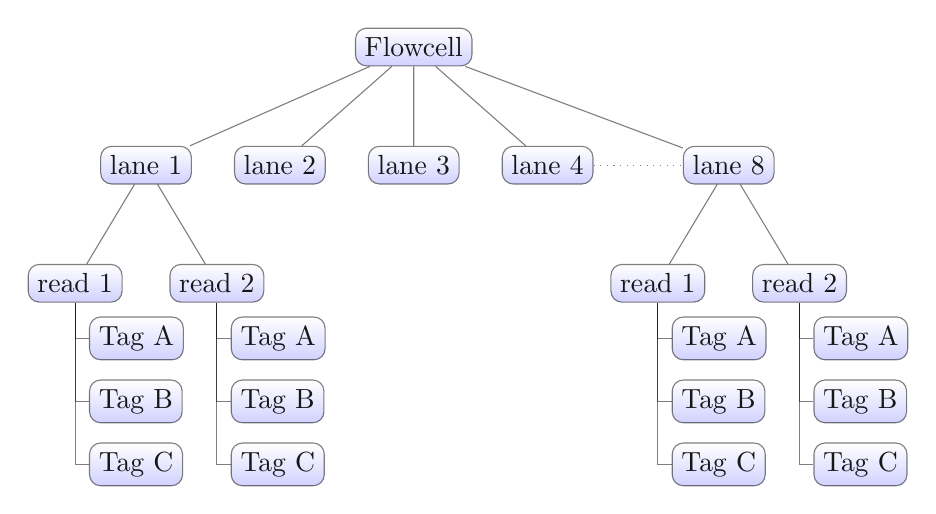
\begin{tikzpicture}[%
	sibling distance=10em,
  	every node/.style = {shape=rectangle, rounded corners,draw,align=center,top color=white, bottom color=blue!20},
    	grandchild/.style={grow=down,xshift=0.5em,anchor=west,
  	  edge from parent path={(\tikzparentnode.south) |- (\tikzchildnode.west)}},
  	grandchildRight/.style={grow=down,xshift=0.5em,anchor=west,
  	  edge from parent path={(\tikzparentnode.south) |-(\tikzchildnode.west)}},
	level 1/.style={sibling distance=17mm},
	level 2/.style={sibling distance=18mm},
	fill opacity=.9,draw opacity=.5
	]
  \node {Flowcell}
    child { node [level 1] (c1) {lane 1}
    		child [level 2] {node {read 1}
    			child [grandchild, level distance=23mm] { node {Tag C}}
    			child [grandchild, level distance=15mm] { node {Tag B}}
    			child [grandchild, level distance=7mm] { node {Tag A}}}
    		child [level 2] {node {read 2}
    			child [grandchildRight, level distance=23mm] { node {Tag C}}
    			child [grandchildRight, level distance=15mm] { node {Tag B}}
			child [grandchildRight, level distance=7mm] { node {Tag A}}
    		}}
    child [level 1] { node {lane 2} }
	child [level 1] { node {lane 3} }
	child [level 1] { node (c4) {lane 4} }
    child [sibling distance=20mm] { node (c8) {lane 8}
		child [level 2] { node {read 1}
			child [grandchild, level distance=23mm] { node {Tag C}}
    			child [grandchild, level distance=15mm] { node {Tag B}}
    			child [grandchild, level distance=7mm] { node {Tag A}}}
    		child [level 2] {node {read 2}
    			child [grandchildRight, level distance=23mm] { node {Tag C}}
    			child [grandchildRight, level distance=15mm] { node {Tag B}}
			child [grandchildRight, level distance=7mm] { node {Tag A}}}
    		};
 \draw [dotted] (c4) -- (c8);
		\end{tikzpicture}
 \caption{The hierachical structure of data at the lowest level, tag level, of measurement.\label{HirStructure}}
\end{figure}
\end{center}
\end{frame}

\begin{frame}\frametitle{Hierachical structure of the data}
\begin{center}
\begin{figure}[!ht]
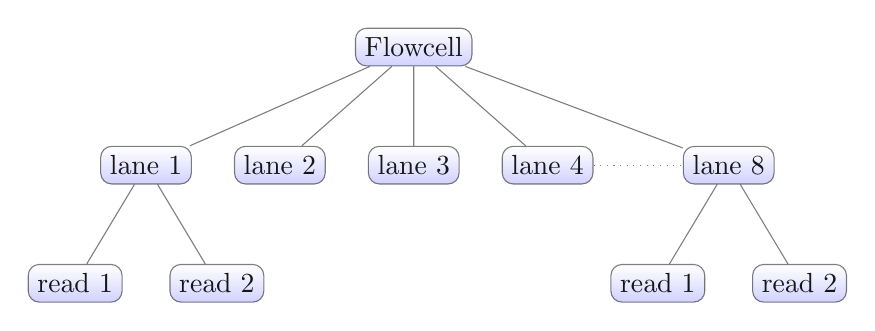
\begin{tikzpicture}[%
	sibling distance=10em,
  	every node/.style = {shape=rectangle, rounded corners,draw,align=center,top color=white, bottom color=blue!20},
    	grandchild/.style={grow=down,xshift=0.5em,anchor=west,
  	  edge from parent path={(\tikzparentnode.south) |- (\tikzchildnode.west)}},
  	grandchildRight/.style={grow=down,xshift=0.5em,anchor=west,
  	  edge from parent path={(\tikzparentnode.south) |-(\tikzchildnode.west)}},
	level 1/.style={sibling distance=17mm},
	level 2/.style={sibling distance=18mm},
	fill opacity=.9,draw opacity=.5
	]
  \node {Flowcell}
    child { node [level 1] (c1) {lane 1}
    		child [level 2] {node {read 1}}
    		child [level 2] {node {read 2}}
    		}
    child [level 1] { node {lane 2}}
	child [level 1] { node {lane 3}}
	child [level 1] { node (c4) {lane 4}}
    child [sibling distance=20mm] { node (c8) {lane 8}
		child [level 2] { node {read 1}}
    		child [level 2] {node {read 2}}
    		};
 \draw [dotted] (c4) -- (c8);
		\end{tikzpicture}
 \caption{The hierachical structure of data at the read level of measurement.}
\end{figure}
\end{center}
\end{frame}

 \begin{frame}\frametitle{Completed run cycles}
 \begin{itemize}
 \item Only data on \textit{completed run cycles}, NOT the actual run setting! 
 \end{itemize}
 \pause

 \textbf{Assumption:}
 \pause
A run (ex. paired end v4) performed on 126 (125+1) cycles can result in \textbf{at most} 125 completed run cycles and \textbf{atleast} 120 completed run cycles.

\textbf{HiSeq 6}: cycle 126 paired end has most data for read level. Will be used for creating profile!
\end{frame}

\subsection{Read level figures}
\begin{frame}\frametitle{Comparing HiSeq machines - 126 cycles paired end.}
\begin{knitrout}
\definecolor{shadecolor}{rgb}{0.969, 0.969, 0.969}\color{fgcolor}\begin{figure}
\includegraphics[width=\maxwidth]{figure/MeanFigure-1} \caption[Figure containing the mean and standard deviation of mean q values in each lane/read]{Figure containing the mean and standard deviation of mean q values in each lane/read.}\label{fig:MeanFigure}
\end{figure}


\end{knitrout}
\end{frame}

\begin{frame}\frametitle{Read level - Spearman correlation matrix}
\begin{knitrout}
\definecolor{shadecolor}{rgb}{0.969, 0.969, 0.969}\color{fgcolor}\begin{figure}
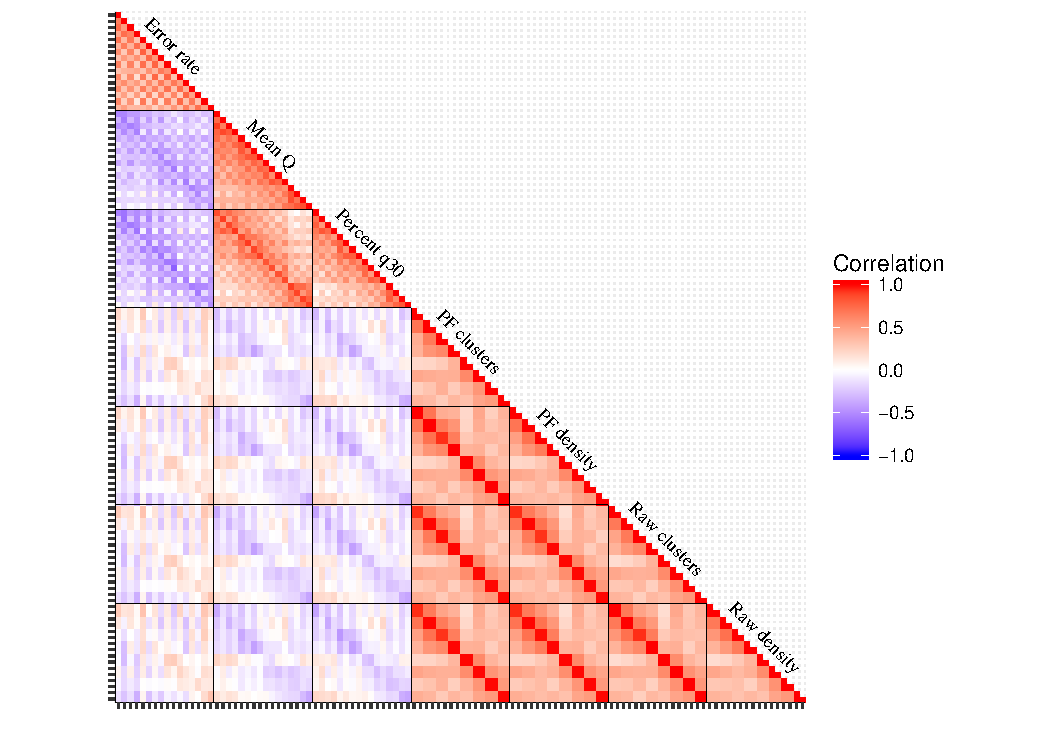
\includegraphics[width=\maxwidth]{figure/ReadlvlCor-1} \caption[Spearman correlation matrix of HiSeq 6 Read level measurements, 126 cycles paired end]{Spearman correlation matrix of HiSeq 6 Read level measurements, 126 cycles paired end}\label{fig:ReadlvlCor}
\end{figure}


\end{knitrout}
\end{frame}
\subsection{Summary of read/tag level measurements}
\begin{frame}\frametitle{Summary}
The structure of the quality control data is very complicated.
\begin{itemize}
\item Want to model at the lowest level (Tag-level). Difference in observations, complicated! Read-level? 
\item The different machine setting provide another complexity to the problem.
\item In terms of mean q, the machines are different! Not true for error rate. 
\item Finding: Percent tag err.= 0 $\rightarrow$ error rate$>0$ in datasets, wrong? 
\end{itemize}
\end{frame}

\subsection{Transformation to normality}
\begin{frame}\frametitle{Modelling - Solution and transform data}

Monitor Read-level! 

Use mean q, error rate and percent q30 for our modelling example.

$$
\mathbf{X} = (X_{mean\_ q\_ 1\_ 1},X_{ErrRate\_ q\_ 1\_ 1},X_{Pctq30\_ q\_ 1\_ 1},X_{mean\_ q\_ 1\_ 2},..., X_{Pctq30\_ q\_ 8\_ 2})
$$

Can the data be assumed to follow a multivariate normal distribution? No... $\rightarrow$ Transform! \textbf{Assume} $\mathbf{X}^*\sim \mathcal{N}_p(\boldsymbol{\mu}_0,\Sigma_0)$.
\end{frame}
 
% \begin{frame}\frametitle{Normality assumption and different transformations}
%  Box-Cox transformation together with Guerro method for variables on positive real line. Box-Cox transformation:
%  $$
%  Y = \begin{cases}
%  \frac{X^{\lambda}-1}{\lambda}, \text{ if } \lambda\neq 0 \\
%  \log X, \text{ else.}
%  \end{cases}
%  $$
%  estimate $\lambda$ using Guerro method. 
%  
% For variables with limited support (i.e. (0,1)) $\rightarrow$ quantile normal function.
% $$ Y = \Phi^{-1}(X)
% $$ where $\Phi^{-1}(\cdot)$ is the standard normal quantile function.
% \end{frame}

\section{Results}
\subsection{Results - Simulation study}
 
\begin{frame}\frametitle{Stress testing}
Simulation study of two different scenarios. How quickly can we detect changes in profile? Will show change in $\boldsymbol{\mu}_0$. 
 \begin{itemize}
 \item Scenario 1. Lane 1 shows worse behaviour (all variables): all change according to $\delta$
 \item Scenario 2. The error rate shows worse performance in lane 1: change according to $\delta$
 \end{itemize}
 \pause
 Performance measures:
 \begin{enumerate}
 \item ARL$_1$ (MCUSUM, Hotelling $T^2$)
 \item Expected delay, 20 profile runs before machine breaks (MCUSUM)
 \end{enumerate}
\end{frame}




\begin{frame}\frametitle{Scenario 1 - All variables, lane 1 change}
\begin{knitrout}
\definecolor{shadecolor}{rgb}{0.969, 0.969, 0.969}\color{fgcolor}\begin{figure}
\includegraphics[width=\maxwidth]{figure/Scenario1mean-1} \caption[Scenario 1]{Scenario 1. ARL1 and ED for the MCUSUM model for different delta. }\label{fig:Scenario1mean}
\end{figure}


\end{knitrout}
Hotelling's did not discover any of the changes (ARL$_1\geq 500$).
\end{frame}

\begin{frame}\frametitle{Scenario 2 - change in the error rate by $\delta$}
\begin{knitrout}
\definecolor{shadecolor}{rgb}{0.969, 0.969, 0.969}\color{fgcolor}\begin{figure}
\includegraphics[width=\maxwidth]{figure/Scenario2mean-1} \caption[Scenario 2]{Scenario 2. ARL1 and ED for the MCUSUM model for different delta.}\label{fig:Scenario2mean}
\end{figure}


\end{knitrout}
Hotelling's did not discover any of the changes (ARL$_1\geq 500$).
\end{frame}

\begin{frame}\frametitle{CPD - estimate change point}
\begin{enumerate}
\item Simulate 20 runs according to profile
\item Simulate the number of runs it took us to discover the change (according to ED)
\item estimate change point (21st run)
\item D = estimated changepoint - simulated changepoint.
\end{enumerate}
Repeat $10^5$ times, take average. 
\end{frame}

\begin{frame}\frametitle{CPD - simulations}
\begin{knitrout}
\definecolor{shadecolor}{rgb}{0.969, 0.969, 0.969}\color{fgcolor}\begin{figure}
\includegraphics[width=\maxwidth]{figure/CPDfig-1} \caption[Offset average estimate of the change-point detection model]{Offset average estimate of the change-point detection model.}\label{fig:CPDfig}
\end{figure}


\end{knitrout}
\end{frame}

\begin{frame}\frametitle{Summary of stress test}
\begin{itemize}
\item Quick to detect change in a whole lane
\item Not so quick to detect changes in one variable. 
\item CPD model, poor for small $\delta$. Result of unbalanced sample?
\end{itemize}
\end{frame}

\subsection{Results - Application on HiSeq quality control data.}

\begin{frame}\frametitle{How do models work in practice}
\begin{itemize}
\item Transform new data according to transformation methods.
\item Use Hotelling + MCUSUM models so see if new data fits profile.
\item Anything above control limit indicates change in profile.
\end{itemize}
\textbf{Note:} Transformation parameters are estimated from HiSeq 6 data and then used to transform HiSeq 3, 4 and 5 data.
\end{frame}


\begin{frame}\frametitle{How do models work - simulated example of Hotelling}
\begin{knitrout}
\definecolor{shadecolor}{rgb}{0.969, 0.969, 0.969}\color{fgcolor}\begin{figure}
\includegraphics[width=\maxwidth]{figure/ExampleHotelling-1} \caption[Example of Hotellings T2 statistic]{Example of Hotellings T2 statistic.}\label{fig:ExampleHotelling}
\end{figure}


\end{knitrout}
\end{frame}
 
\begin{frame}\frametitle{Hotelling's $T^2$ statistic}
\begin{knitrout}
\definecolor{shadecolor}{rgb}{0.969, 0.969, 0.969}\color{fgcolor}\begin{figure}
\includegraphics[width=\maxwidth]{figure/HotellingsPicture-1} \caption[Hotellings T statistic for HiSeq 3, 4 and 5]{Hotellings T statistic for HiSeq 3, 4 and 5. HiSeq 3 has no paired end 126 cycle runs!}\label{fig:HotellingsPicture}
\end{figure}


\end{knitrout}
\end{frame}



\begin{frame}\frametitle{MCUSUM - HiSeq 4 and 5 cycle 126 paired end.}
\begin{knitrout}
\definecolor{shadecolor}{rgb}{0.969, 0.969, 0.969}\color{fgcolor}\begin{figure}
\includegraphics[width=\maxwidth]{figure/MCUSUMmean1-1} \caption[MCUSUM model for the mean tested on transformed HiSeq 4 and 5 data]{MCUSUM model for the mean tested on transformed HiSeq 4 and 5 data.}\label{fig:MCUSUMmean1}
\end{figure}


\end{knitrout}
\end{frame}
 
 \section{Summary}
 \begin{frame}\frametitle{Summary}
 \begin{itemize}
 \item Constructed two models for detecting transient and large or persistent and small changes. CPD model for estimating change-points.
 \begin{itemize}
 \item Persistent changes in mean presented here. 
 \item Covariance is also considered in thesis.
 \end{itemize}
 \item Constructed models detect changes in the mean and covariance for all HiSeq machines. Why? \pause
 Probably transformation or possibly not the same quality on average!
 \item Trends? Can be read from the MCUSUM model. 
 \end{itemize}
 \end{frame}

 \section{Discussion}
 \begin{frame}\frametitle{Assumptions and complications with the suggested methods}
 \begin{itemize}
 \item Assumptions of normality and independence, are they violated? Short answer, yes. Implications?
 \pause
 \begin{itemize}
 \item MCUSUM: Control limit may be too small/large, ARL$_0$/ARL$_1$ misspecified. Solution?
 \item Hotellings: Robust against deviations of the assumption of normality. 
 \end{itemize}
\item Dependence between runs, different settings (High output/rapid, single/paired end) $\rightarrow$ create profile for each setting. Solution? 
 \end{itemize}
 
 \end{frame}

 \begin{frame}\frametitle{Other methods?}
 \begin{itemize}
 \item Non-parametric multivariate methods, have not found any methods on specifying the control limits except for bootstrap based (need large data sets, we have small sets.)
 \item Reinforcement learning could work but also demand large data sets.
 \end{itemize}
 \end{frame}

\begin{frame}
\begin{center}
{\Large Thank you!} 
\newline
\end{center}
Thanks to the SNP\&SEQ platform for giving me this opportunity, my supervisor Johan D. for his support/guidance and last all of those who have helped me in this process! 
\end{frame}

\section{Optional - MATH!}

\begin{frame}\frametitle{Hotelling's $T^2$ statistic}
Let $\mathbf{X}_t$ be the $t$'th observation. Under the null hyp. $\mathbf{X}_t \sim \mathcal{N}_p(\boldsymbol{\mu}_0,\Sigma_0)$, and let
$$
T^2_{2,t} = (\mathbf{X}_t-\boldsymbol{\mu}_0)'\boldsymbol{\Sigma}^{-1}_0(\mathbf{X}_t-\boldsymbol{\mu}_0).
$$ 
then
$$
\frac{(M-p)M}{p(M-1)(M+1)} T^2_{2,t} \sim \mathcal{F}_{p,M-p}
$$
if 
$$
T^2_{2,t}>\frac{p(M-1)(M+1)}{(M-p)M}\mathcal{F}_{p,M-p}$$
signal change!
\end{frame}

\begin{frame}\frametitle{MCUSUM statistic}
Let $\mathbf{S}_0=\mathbf{0}$ and then. 
\begin{align}
&C_t=\sqrt{(\mathbf{S}_{t-1}+\mathbf{X}_t-\boldsymbol{\mu}_0)'\boldsymbol{\Sigma}^{-1}_0
(\mathbf{S}_{t-1}+\mathbf{X}_t-\boldsymbol{\mu}_0)}\label{MCUSUM} &\\ 
&\mathbf{S}_t=\begin{cases}
\mathbf{0} & \text{if} \; C_t \leq k \\
(\mathbf{S}_{t-1}+\mathbf{X}_t-\boldsymbol{\mu}_0)(1-k/C_t) & \text{otherwise}
\end{cases} \label{MCUSUM2} &
\end{align}
where $k$ is the allowance constant. Let 
\begin{equation}\label{Ht}
H_t=\sqrt{\mathbf{S}_t'\boldsymbol{\Sigma}^{-1}_0 \mathbf{S}_t},
\end{equation} 
if $H_t>h$ signal a change.
\end{frame}

\end{document}

% 
% \begin{description}[align = right]
%  \item Problem:
% \end{description}
% \end{frame}
